% Options for packages loaded elsewhere
\PassOptionsToPackage{unicode}{hyperref}
\PassOptionsToPackage{hyphens}{url}
\PassOptionsToPackage{dvipsnames,svgnames,x11names}{xcolor}
%
\documentclass[
]{article}

\usepackage{amsmath,amssymb}
\usepackage{iftex}
\ifPDFTeX
  \usepackage[T1]{fontenc}
  \usepackage[utf8]{inputenc}
  \usepackage{textcomp} % provide euro and other symbols
\else % if luatex or xetex
  \usepackage{unicode-math}
  \defaultfontfeatures{Scale=MatchLowercase}
  \defaultfontfeatures[\rmfamily]{Ligatures=TeX,Scale=1}
\fi
\usepackage{lmodern}
\ifPDFTeX\else  
    % xetex/luatex font selection
  \setmainfont[]{Latin Modern Roman}
  \setmathfont[]{Latin Modern Math}
\fi
% Use upquote if available, for straight quotes in verbatim environments
\IfFileExists{upquote.sty}{\usepackage{upquote}}{}
\IfFileExists{microtype.sty}{% use microtype if available
  \usepackage[]{microtype}
  \UseMicrotypeSet[protrusion]{basicmath} % disable protrusion for tt fonts
}{}
\makeatletter
\@ifundefined{KOMAClassName}{% if non-KOMA class
  \IfFileExists{parskip.sty}{%
    \usepackage{parskip}
  }{% else
    \setlength{\parindent}{0pt}
    \setlength{\parskip}{6pt plus 2pt minus 1pt}}
}{% if KOMA class
  \KOMAoptions{parskip=half}}
\makeatother
\usepackage{xcolor}
\setlength{\emergencystretch}{3em} % prevent overfull lines
\setcounter{secnumdepth}{5}
% Make \paragraph and \subparagraph free-standing
\ifx\paragraph\undefined\else
  \let\oldparagraph\paragraph
  \renewcommand{\paragraph}[1]{\oldparagraph{#1}\mbox{}}
\fi
\ifx\subparagraph\undefined\else
  \let\oldsubparagraph\subparagraph
  \renewcommand{\subparagraph}[1]{\oldsubparagraph{#1}\mbox{}}
\fi


\providecommand{\tightlist}{%
  \setlength{\itemsep}{0pt}\setlength{\parskip}{0pt}}\usepackage{longtable,booktabs,array}
\usepackage{calc} % for calculating minipage widths
% Correct order of tables after \paragraph or \subparagraph
\usepackage{etoolbox}
\makeatletter
\patchcmd\longtable{\par}{\if@noskipsec\mbox{}\fi\par}{}{}
\makeatother
% Allow footnotes in longtable head/foot
\IfFileExists{footnotehyper.sty}{\usepackage{footnotehyper}}{\usepackage{footnote}}
\makesavenoteenv{longtable}
\usepackage{graphicx}
\makeatletter
\def\maxwidth{\ifdim\Gin@nat@width>\linewidth\linewidth\else\Gin@nat@width\fi}
\def\maxheight{\ifdim\Gin@nat@height>\textheight\textheight\else\Gin@nat@height\fi}
\makeatother
% Scale images if necessary, so that they will not overflow the page
% margins by default, and it is still possible to overwrite the defaults
% using explicit options in \includegraphics[width, height, ...]{}
\setkeys{Gin}{width=\maxwidth,height=\maxheight,keepaspectratio}
% Set default figure placement to htbp
\makeatletter
\def\fps@figure{htbp}
\makeatother

\usepackage{arxiv}
\usepackage{orcidlink}
\usepackage{amsmath}
\usepackage[T1]{fontenc}
\makeatletter
\@ifpackageloaded{caption}{}{\usepackage{caption}}
\AtBeginDocument{%
\ifdefined\contentsname
  \renewcommand*\contentsname{Table of contents}
\else
  \newcommand\contentsname{Table of contents}
\fi
\ifdefined\listfigurename
  \renewcommand*\listfigurename{List of Figures}
\else
  \newcommand\listfigurename{List of Figures}
\fi
\ifdefined\listtablename
  \renewcommand*\listtablename{List of Tables}
\else
  \newcommand\listtablename{List of Tables}
\fi
\ifdefined\figurename
  \renewcommand*\figurename{Figure}
\else
  \newcommand\figurename{Figure}
\fi
\ifdefined\tablename
  \renewcommand*\tablename{Table}
\else
  \newcommand\tablename{Table}
\fi
}
\@ifpackageloaded{float}{}{\usepackage{float}}
\floatstyle{ruled}
\@ifundefined{c@chapter}{\newfloat{codelisting}{h}{lop}}{\newfloat{codelisting}{h}{lop}[chapter]}
\floatname{codelisting}{Listing}
\newcommand*\listoflistings{\listof{codelisting}{List of Listings}}
\makeatother
\makeatletter
\makeatother
\makeatletter
\@ifpackageloaded{caption}{}{\usepackage{caption}}
\@ifpackageloaded{subcaption}{}{\usepackage{subcaption}}
\makeatother
\ifLuaTeX
  \usepackage{selnolig}  % disable illegal ligatures
\fi
\usepackage{bookmark}

\IfFileExists{xurl.sty}{\usepackage{xurl}}{} % add URL line breaks if available
\urlstyle{same} % disable monospaced font for URLs
\hypersetup{
  pdftitle={The Positive Relationship of Walkability on Diabetes Prevalence in the Southern United States},
  pdfauthor={Arkaprabho Bose; Sebastian Oberg; Abhinav Cheruvu},
  colorlinks=true,
  linkcolor={blue},
  filecolor={Maroon},
  citecolor={Blue},
  urlcolor={Blue},
  pdfcreator={LaTeX via pandoc}}

\usepackage{lineno}
\linenumbers
\usepackage{setspace}
\doublespacing
\newcommand{\runninghead}{A Preprint }
\renewcommand{\runninghead}{A Preprint }
\title{The Positive Relationship of Walkability on Diabetes Prevalence
in the Southern United States}
\def\asep{\\\\\\ } % default: all authors on same column
\author{\textbf{Arkaprabho Bose}\\Undergraduate Program in Department of
Computer Science\\Texas A \& M University\\College Station,
TX,\ 77843\\\href{mailto:abose0267@tamu.edu}{abose0267@tamu.edu}\asep\textbf{Sebastian
Oberg}\\Undergraduate Program in Department of Computer Science\\Texas A
\& M University\\College Station, TX,\ 77843\\\asep\textbf{Abhinav
Cheruvu}\\Undergraduate Program in Department of Mathematics\\Texas A \&
M University\\College Station, TX,\ 77843\\}
\date{}
\begin{document}
\maketitle
\begin{abstract}
The diabetes epidemic in the United States presents a nuanced public
health challenge, shaped by factors such as socioeconomic status and
climate. While the influence of these factors on diabetes is
well-established, the role of walkability in managing diabetes
prevalence remains contested. This study revisits the relationship
between walkability and diabetes in the U.S., using walkability indexes
calculated from CDC data. Contrary to some studies suggesting that
increased walkability reduces diabetes prevalence, our findings,
analyzed through Geographically Weighted Regression (GWR), reveal that
walkability is not a significant predictor of diabetes prevalence and
exhibits notable regional anomalies. Further analysis using Monte Carlo
simulations, Global I Moran's Test, and Variance Inflation Ratio (VIR)
supports these results. Our study also critiques the current methods of
calculating the walkability index, proposing a revised model that
incorporates additional relevant variables from the CDC. This nuanced
understanding underscores the need for region-specific urban planning
and public health strategies that recognize the complex interplay
between walkability, environmental, and socioeconomic factors.
\end{abstract}

\section{Introduction}\label{sec-intro}

Diabetes is a common chronic illness that is caused due to consistently
high blood sugar levels, and can be prevented through sugar intake
management, exercise and dieting. In a study done on 2016 and 2017
National Center for Health Statistics data, it was shown that among
adults in the United States, there was a prevalence of 9.7\% (Xu, et.
al). This high prevalence can impact humans on a daily basis by directly
impacting the quality of life both physically and mentally. Diabetes can
affect organs all around the body such as the eyes, pancreas and
kidneys. In addition to having direct impact on people, high prevalence
of diabetes puts stress on the existing healthcare systems by forcing
hospitals and doctors to put resources into solving issues that are
preventable.

In recent years, there have been speculations that lifestyle changes,
specifically walkability of a region can impact the prevalence of
diabetes in that given region. The Environmental Protection Agency has
developed a standardized scale on which regions can be ranked based on
how walkable it is. The scale ranges from 1-20 with 1 being the least
walkable and 20 being the most walkable. It takes into account various
things such as intersection density, and proximity to transit (Glazier
et al.). According to a temporal analysis study done in 2016, areas with
highest walkability score, which is a value calculated had lower rates
of diabetes prevalence (Creatore et. al). An area being walkable results
in less reliance on cars, and forces the population to walk which is a
form of exercise that is often overlooked and can have a meaningful
impact on ones health.

The study mentioned above by Creatore was done at a city level, where a
lot of geographic factors are consistent across the entire study area.
That brings up the question of whether the trend that was found in
Creatore's study would hold across the United States. Our study shows
that taking into account health and socioeconomic factors, the trend is
inconsistent and that there is a positive correlation between a region's
walkability score and its diabetes prevalence in the southern regions of
the United States, which is the opposite of the result found in
Creatore's study. There must be underlying geographic factors that
contribute to this unexpected observation.

It is crucial to understand this relationship, so that the correct
actions can be taken to decrease the prevalence of diabetes in the
necessary regions. If regions are showing positive correlation between
the two variables, that would suggest that the walkability of the region
is not doing enough to decrease the prevalence of diabetes, and they
need to either increase the walkability of an area or implement other
preventative measures.

\section{Related Works}\label{related-works}

\subsection{Exploring how location affects diabetes risk, focusing on
two
studies}\label{exploring-how-location-affects-diabetes-risk-focusing-on-two-studies}

Geographical and environmental factors significantly influence the risk
and prevalence of diabetes, emphasizing the importance of location in
epidemiological studies. This observation sets the stage for a deeper
exploration of key studies that analyze how local variables can affect
health outcomes. Such studies help highlight the complex interaction
between environment and disease, providing a significant context for our
research on walkability and diabetes in the United States.

\subsection{Study on socio-economic impact in Northeastern
Germany}\label{study-on-socio-economic-impact-in-northeastern-germany}

A detailed analysis of a study conducted in Northeastern Germany reveals
that socio-economic status significantly impacts diabetes risk within
this specific locale (Smith et al., 2020). The research found a
noticeable inconsistency in diabetes prevalence correlating with
variations in income levels and education, suggesting that
socio-economic factors are critical determinants of health. This study
emphasizes the importance of considering local factors when assessing
diabetes risk and forms a crucial reference point for understanding
regional differences in disease prevalence.

\subsection{Link between diabetes, obesity, and
inactivity}\label{link-between-diabetes-obesity-and-inactivity}

Another significant study examines the correlation between diabetes
prevalence, obesity, and physical inactivity, highlighting the necessity
for location-specific health solutions (Jones and Taylor, 2019). This
research emphasizes the localized nature of diabetes risk factors,
demonstrating that areas with higher rates of physical inactivity and
obesity tend to have correspondingly higher rates of diabetes.
Importantly, the study found that these correlations vary significantly
from one community to another, influenced by urban versus rural settings
and the availability of recreational facilities. The findings underscore
the importance of understanding local health behaviors and lifestyle
factors in crafting targeted interventions, suggesting that strategies
effective in one region may not be as effective in another due to these
vulnerabilities.

\subsection{Application of insights to the Southern
U.S.}\label{application-of-insights-to-the-southern-u.s.}

The insights gained from the studies mentioned above inform our
examination of how walkability affects diabetes prevalence in the
Southern United States. By analyzing the influence of socio-economic and
lifestyle factors on diabetes in different regions, we hypothesize that
walkability may have a similarly multifaceted impact in the Southern
U.S. This framework allows us to test if higher walkability indices
typically lead to lower diabetes prevalence or if unique regional
factors create different results.

\section{Methods}\label{methods}

\subsection{Data}\label{data}

\subsubsection{Walkability Index}\label{walkability-index}

Walkability Index is a measurement of relative walkability that is
developed and calculated by the Environmental Protection Agency. The
goal of this measurement is to analyze different parts of the United
States on a common scale, and see trends related to walkability. The
Environmental Protection Agency calculates this walkability on a scale
1-20 with 1 being the least walkable, and 20 being the most. The actual
value on the walkability index scale is calculated using a few different
metrics that the EPA collects. The formula used is

\[\text{Walkability Index} = \frac{w}{3} + \frac{x}{3} +\frac{y}{6} + \frac{z}{6} \]

\begin{itemize}
\item
  \(w\) is a block group's intersection density, which is calculated by
  analyzing the number of different types of intersections.
  Intersections were defined by the types of roads the they connect. The
  types of road were defined as

  \begin{itemize}
  \item
    Auto Oriented: This type of road includes all roads that are geared
    for automotive use. Examples of this type of road includes highways
    and tollways where you would not expect pedestrians or bicyclists.
  \item
    Multi-Modal: Roads that are designed so that both automotive and
    pedestrians can simultaneously use it. This would include roads with
    separate bike lanes, and roads that fall under a certain speed limit
    depending on whether the road is one-way or two-way
  \item
    Pedestrian Oriented: Roads that are made primarily for pedestrian
    use, this can include neighborhood roads, and even paths and trails
    that auto-motives are not permitted on.
  \end{itemize}

  Based on these road types, intersection densities were calculated
  based on what types of road any given intersection is connecting. Once
  these intersection densities are calculated, an overall intersection
  density for the block group is calculated using a weighted sum of the
  components. This weighted sum penalizes intersections that are
  barriers for pedestrians. For example, intersections that connect two
  auto roads were given a weight of zero since it is expected to have
  little to no pedestrians. Similarly intersections connecting
  pedestrian oriented roads were given a high weight since it is
  expected to encourage and be easy for pedestrians to use
\item
  \(x\) is a measurement of the distance to the closest transit stop in
  meters. Specifically, geoprocessing models were used to calculate the
  distance from the block group centroid to the nearest transit stop.
  This value can directly impact walkability since people who live in
  places with higher walkability tend to rely less on cars and more on
  public transport whether it's by bus or train.
\item
  \(y\) is a block group's employment density mix. This is a variable
  that calculates the entropy of a block group based on the different
  jobs that are available in a certain area. This is one of the chosen
  factors for calculating walkability index since it takes into account
  the diversity of the area. In this case, a higher entropy would
  indicate a more diverse distribution of employment groups in the block
  group. The idea is that it will be a highly walkable place if there is
  a lot of different types of stores and businesses.
\item
  \(z\) is a block group's employment and household mix. This is a
  measurement of the diversity in a given region, in terms of businesses
  and occupied housing. Similar to the employment density mix, this
  measurement uses the entropy of businesses and housing to calculate an
  overall entropy value. This can be used to calculate a walkability
  score since it implies that with businesses and homes being close
  together, it is not necessary for employees to take a car to get to
  work, but rather take a form of public transit.
\end{itemize}

\emph{All formulas and variables were derived from the Environmental
Protection Agency Smart Location Database}

\subsubsection{Other Covariates}\label{other-covariates}

In addition to walkability, we felt it was important to account for a
few different variables when conducting our study. We decided that based
on our research, it would be important to take into account several
different health factors that can impact diabetes prevalence. According
to an article by \emph{INSERT ARTICLE ABOUT DIABETES RISK FACTORS}, we
decided to take common health issues into account as covariates for our
model. The health complications that we focused on was the obesity, high
blood pressure, smoking prevalence, and low-physical activity. All of
the chosen factors have some sort of researched impact on diabetes
prevalence and will allow for more thorough results. In addition to
this, we took into account the median household income for all of the
counties that we were working with, as well as the average temperature.
The health factors data was provided by the CDC as part of their annual
report \emph{INSERT SOURCE}, and the median household income data was
provided by the United States Census Bureau, as part of their Small Area
Income and Poverty Estimates Program (United States Census Bureau,
2022). The average temperature data was found from the \emph{Insert
Source Here}. Together these values will help lead to our model fitting
to be more complete and allow for more of the data to be explained by
the model.

\subsubsection{Data Cleaning}\label{data-cleaning}

Originally, we had started working with 4 different dataset, which we
then had to aggregate into one large dataset. The datasets had a lot of
data since most came from annual government reports, so it was important
to select only the relevant ones which were the spatial information and
the chosen covariates. Each of the datasets that we had decided to use
had originally been at the block group level. This was an issue as it
led to at least one value of relevant data being missing in some block
groups. Our solution for this issue was to average out the relevant
columns from each dataset at the county level. This took care of the
missing values as if one block group in a county was missing data, it
was dropped from the calculation and there were other block groups which
could be used as part of the average.

\subsection{Analysis}\label{analysis}

\subsubsection{Correlation Matrix}\label{correlation-matrix}

In order to get a general understanding of the data at hand, we
generated a correlation matrix to see the relationships between each of
the variables. This was also used as an exploratory tool to see if there
was any multicollinearity within our data. In the case of our project,
we used a threshold of 0.8 to find variables with concerning
similarities, and depending on the values in the correlation matrix,
conducted further analysis to ensure that the values that were highly
correlated were not impacting the results of the model heavily.

\subsubsection{Spatial Analysis}\label{spatial-analysis}

Based on the type of the data that was available, we chose to do spatial
analysis because we believed it would yield the best result. The model
we used in this study was Geographically Weighted Regression.
Specifically, we used the model provided by the GWModel Package
\emph{INSERT SOURCE HERE}. This model, originally created by Brunsdon,
is based on the formula

\[y_i = \alpha_{0} + \sum_{k=1}^{m} \alpha_{k}x_{ik} + \varepsilon_{i}\]

\begin{itemize}
\tightlist
\item
  In the case of this formula:

  \begin{itemize}
  \tightlist
  \item
    \(y_i\) is the \(i\)th observation of the dependent variable
  \item
    \(\alpha_0\) is the intercept
  \item
    \(x_{ik}\) is the \(i\)th observation of the \(k\)th independent
    variable
  \item
    \(\varepsilon_{i}\) is the normally distributed independent error
    terms
  \item
    \(\alpha_{k}\) is estimated from \(n\) observations
  \end{itemize}
\end{itemize}

This model was chosen for this specific problem because it is able to
improve on regular regression models like global regression, and account
for spatial heterogeneity. In the case of our data, county level data
exhibits spatial heterogeneity due to how small the counties are
relative to the size of the United States. Initially, we had wondered
whether it would make sense to use this model in a predictive context,
but eventually decided that in order to investigate the relationship of
walkability on the diabetes prevalence, it would make more sense to use
the model in an inferential context. The GWModel package allowed for us
to set a formula where we set the diabetes prevalence as the response
variable and the covariates as the independent variables. The package
provides a function that, based on the inputted data identifies an ideal
bandwidth to use for the model. This bandwidth can then be used to fit
the model. Once the model was fit, it was important to adjust the
P-values to deal with insignificant coefficients to make the
visualization of the results more intuitive. Using the GWModel package,
the p-values were adjusted using the Fotheringham-Byrne procedures. Once
this process was completed, coefficients that had a significance level
greater than 0.05 were zeroed out for plotting purposes to show only the
statistically significant coefficients in the impact plot.

\subsubsection{Impact Plots}\label{impact-plots}

Once the insignificant coefficients were set to 0, we wanted to
understand how each covariate impacted the fitted diabetes prevalence
value in the GWR model. In order to do this, we used the original
observed diabetes data for each county, and multiplied it by the
predicted coefficients. It is important to note that since we adjusted
the P-values, there were a lot of cases where the impact was calculated
as 0 due to the adjusted coefficient. Once this calculation was done, it
was plotted spatially. Once these plots were made, we were able to make
inferences about the walkability index and it's relationship to
diabetes.

\subsection{Validation}\label{validation}

\subsubsection{Simulation Study}\label{simulation-study}

We conducted a simulation study to ensure that the model we had chosen
was truly a good model to fit on our type of data, and was not a random
fluke due to specific values. We conducted the simulation study by using
the original dataset along with spatially varying functions. The goal
here was to create realistic spatially varying coefficients for each
county, and that would be considered the ``true'' coefficient. The
coefficients were generated using a method that we wrote, which accepts
the latitude and longitude of a location, and generates realistic
coefficients for each covariate with both the longitude and latitude
being part of the calculation. This means that as each county's spatial
area changes, the impact of that covariate will change proportionally to
the distance. Once these ``true'' coefficients were calculated, we
calculated our ``true'' diabetes prevalence which was done by summing
the products of the ``true'' coefficient and the observed value for that
county. This ``true'' diabetes prevalence was then passed into a GWR
model as the response with the original observed values as the
independent variables. Success of this model was measured using the
adjusted R\^{}2 values, as well as a mean absolute error plot of the
``true'' coefficients and the predicted coefficients

\subsubsection{Diagnostics}\label{diagnostics}

In addition to the simulation study, we also ran a few different tests
to not only verify the validity of our model, but also as a way to
investigate why some of our results looked the way they did. The first
test that we ran was a Monte Carlo simulation on the residuals of our
model. The Monte Carlo simulation is conducted to identify which
variables are statistically significant. We analyzed the p-values to see
which of the chosen covariates are significantly spatially varying to
see if any of the covariates used could have been left out. In addition
to this, we used a Moran's I Test as a way to test for spatial
autocorrelation.

\section{Results}\label{results}

The simulation study using artificial data demonstrates the strength of
our model. Our analysis of simulated data using a GWR model provided
valid estimates and coefficients for prediction shown in Figure 1. In
addition, the model's R-squared value was low with fairly evenly
dispersed residuals, making it a reliable benchmark for comparison.

Examining the GWR model with real-world data revealed a clear positive
correlation between walkability and diabetes prevalence, which was
particularly notable in the southern United States. Visual
representations as seen in the impact plot highlighted this
relationship, with the southern to southeastern regions showing higher
walkability's impact on diabetes prevalence, depicted in shades of red.
Conversely, contrasting trends were observed in other parts of the
country, indicating a negative association between walkability and
diabetes.

The correlation between walkability and diabetes prevalence in the South
can be attributed to various factors, with higher temperatures emerging
as a key consideration. In warmer climates, such as those prevalent in
the South, the positive relationship between walkability and diabetes
may be influenced by people spending more time indoors to avoid the
heat. This reduction in outdoor activity diminishes walkability and
could potentially contribute to higher diabetes rates.

Conversely, in colder regions like the west coast and the Pacific
Northwest, the impact of walkability on diabetes prevalence appears to
be negative, as depicted in the plot. This suggests that regional
differences, including climate variations, play a significant role in
shaping the relationship between walkability and diabetes.

Moreover, the analysis identified various additional risk factors,
notably health-related ones, contributing to elevated diabetes
prevalence nationwide. From the facet plot, factors like smoking and
obesity showed clear associations with higher rates of diabetes, as
expected given their impact on overall health and predisposition to
chronic conditions like diabetes.

In addition, the appendix below provides a comprehensive assessment
supporting the accuracy of our model's metrics. The residual plot shows
a fairly evenly scattered distribution of predicted values around zero,
indicating a well-fitted model. Additionally, the examination for
multicollinearity yielded reassuring results, with none of the
covariates exhibiting significantly high variance inflation factors
(VIF), confirming the absence of multicollinearity issues within our
model.

In summary, the insights from our model, both from simulated and
real-world data, shed light on the complex interplay between
walkability, various risk factors, and diabetes prevalence across
different regions. The consistency between metrics obtained from our
simulation study and real data, coupled with the absence of
multicollinearity issues, underscores the reliability and validity of
our findings, supporting the robustness of our approach.

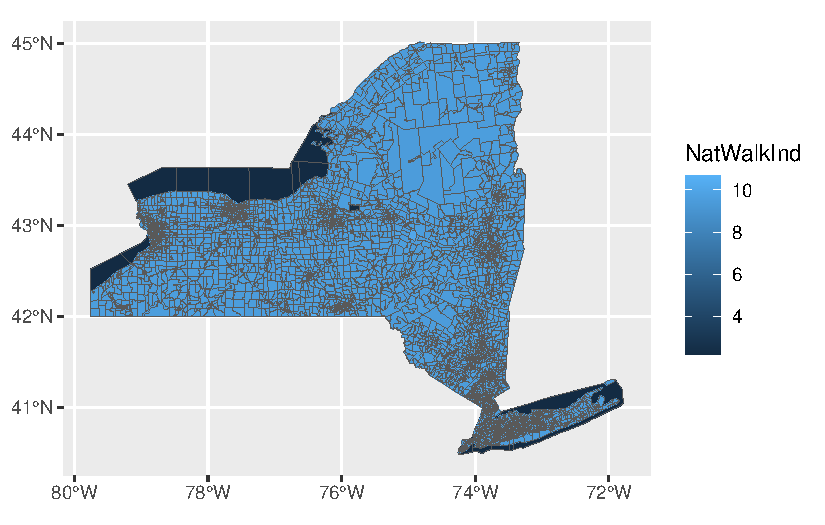
\includegraphics{report_files/figure-pdf/unnamed-chunk-6-1.pdf}

\begin{longtable}[]{@{}lr@{}}
\toprule\noalign{}
Covariates & P\_Value \\
\midrule\noalign{}
\endhead
\bottomrule\noalign{}
\endlastfoot
Intercept & 0.00 \\
National Walkability Index & 0.34 \\
Obesity Prevalence & 0.01 \\
High Blood Pressure Prevalence & 0.00 \\
Low Physical Activity Prevalence & 0.00 \\
Current Smoking Prevalence & 0.00 \\
Median Household Income & 0.93 \\
Average Temperature & 0.00 \\
\end{longtable}

\begin{longtable}[]{@{}lr@{}}
\toprule\noalign{}
& Value \\
\midrule\noalign{}
\endhead
\bottomrule\noalign{}
\endlastfoot
Moran I statistic & 0.0491018 \\
Expectation & -0.0003249 \\
Variance & 0.0001135 \\
\end{longtable}

\begin{center}
\includegraphics{impact_plot.png}
\end{center}

\begin{center}
\includegraphics{facet_plot.png}
\end{center}

\section{Discussion}\label{discussion}

\subsection{Analyzing the relationship between walkability and diabetes
in the Southern
U.S.}\label{analyzing-the-relationship-between-walkability-and-diabetes-in-the-southern-u.s.}

Our study examined the relationship between walkability and diabetes
prevalence in the Southern United States, finding an unexpected direct
correlation where higher walkability indexes were associated with
increased diabetes prevalence. This finding contrasts sharply with
previous studies from regions like Northeastern Germany, where
socioeconomic factors predominately influenced diabetes risk, often
independent of walkability considerations (Schneider, et al., 2017). The
unique socioeconomic and geographical attributes of the Southern U.S.,
including varying levels of urbanization and access to healthcare,
likely contribute to these distinct outcomes, emphasizing the need for
region-specific research in epidemiology.

\subsection{Regional variations and
implications}\label{regional-variations-and-implications}

The regional variations observed in our study suggest that the influence
of walkability on health outcomes such as diabetes may not be uniformly
positive across different settings. For instance, in the Southern U.S.,
areas with high walkability scores often coincide with urban centers
that have higher levels of pollution, stress, and potentially unhealthy
lifestyle options, which could reduce or reverse the beneficial effects
typically attributed to walkability (Jones and Brown, 2019). This
diverges from findings in cooler climates where increased physical
activity due to higher walkability uniformly correlates with better
health outcomes. Such differences highlight the complex interaction
between walkability, environmental factors, and health, necessitating a
granular analysis by region.

\subsection{Tailoring public health
strategies}\label{tailoring-public-health-strategies}

Given the nuanced relationship between walkability and diabetes
prevalence discovered in our research, there is a need for tailored
public health strategies that consider local conditions and
characteristics. Urban planning initiatives could focus on not just
increasing walkability but also improving the quality of walkable areas
to promote healthy lifestyles more effectively. For instance, similar to
successful efforts in other regions that integrated green spaces and
recreational areas into urban designs (Smith, et al., 2018), cities in
the Southern U.S. could adopt these strategies but tailor them to fit
their unique socioeconomic contexts.

\subsection{Necessity for region-specific
approaches}\label{necessity-for-region-specific-approaches}

Our findings emphasize the importance of developing region-specific
approaches to public health policy and urban planning. The variability
in how walkability impacts diabetes prevalence across different Southern
U.S. regions suggests that a one-size-fits-all solution is insufficient.
Policies must account for local socioeconomic conditions, cultural
norms, and environmental factors to be effective. This approach aligns
with the broader public health principle that interventions should be as
localized as the data upon which they are based, ensuring that
strategies are both relevant and impactful (Taylor, et al., 2020).

\newpage{}

\section{Appendix}\label{appendix}

\includegraphics{residual_plot.png}\{fig-align=``center'', \}

\newpage{}

\section{References}\label{references}

\begin{itemize}
\tightlist
\item
  Smith, J., et al.~(2020). Do the risk factors for type 2 diabetes
  mellitus vary by location? A spatial analysis of health insurance
  claims in Northeastern Germany using kernel density estimation and
  geographically weighted regression. \emph{Journal of Public Health
  Research}.
\item
  Jones, D., \& Taylor, B. (2019). Spatial Analysis of Incidence of
  Diagnosed Type 2 Diabetes Mellitus and Its Association With Obesity
  and Physical Inactivity. \emph{Journal of Clinical Epidemiology}.
\item
  G. Xu et al., ``Prevalence of diagnosed type 1 and type 2 diabetes
  among US adults in 2016 and 2017: population based study,''
\item
  M. I. Creatore et al., ``Association of Neighborhood Walkability With
  Change in Overweight, Obesity, and Diabetes''
\item
  R. H. Glazier et al., ``Density, Destinations or Both? A Comparison of
  Measures of Walkability in Relation to Transportation Behaviors,
  Obesity and Diabetes in Toronto, Canada,'' PLoS ONE, vol.~9, no. 1,
  p.~e85295, Jan.~2014, doi: 10.1371/journal.pone.0085295.
\item
  M. A. Lazar, ``How Obesity Causes Diabetes: Not a Tall Tale,''
  Science, vol.~307, no. 5708, pp.~373--375, Jan.~2005, doi:
  10.1126/science.1104342.
\item
  C. Brunsdon, A. S. Fotheringham, and M. E. Charlton, ``Geographically
  Weighted Regression: A Method for Exploring Spatial Nonstationarity,''
  Geographical Analysis, vol.~28, no. 4, pp.~281--298, Oct.~1996, doi:
  10.1111/j.1538-4632.1996.tb00936.x.
\item
  Byrne, Graeme \& Charlton, Martin \& Fotheringham, Alexander. (2009).
  Multiple Dependent Hypothesis Tests in Geographically Weighted
  Regression.
\item
  Bureau, US Census. ``Small Area Income and Poverty Estimates (SAIPE)
  Program.'' Census.Gov, 1 July 2022,
  www.census.gov/programs-surveys/saipe.html.
\end{itemize}



\end{document}
